\documentclass[runningheads, a4paper]{llncs}
\usepackage{graphicx}
\usepackage{amsmath,amssymb,amsfonts}
\usepackage{algorithmic}
\usepackage{textcomp}
\usepackage{xcolor}
\usepackage{hyperref}
\usepackage{listings}
\usepackage{tikz}
\usetikzlibrary{shapes.geometric, arrows, positioning}

% Disable hyphenation
\tolerance=1
\emergencystretch=\maxdimen
\hyphenpenalty=10000
\hbadness=10000

\begin{document}

\title{HumaLity: An Advanced Ensemble-Based AI Text Humanization and Detection Platform}
\titlerunning{HumaLity: Advanced AI Text Humanization and Detection}

\author{Chetas Parekh \and Arric Sekhon \and Swastik Amatya}
\authorrunning{C. Parekh et al.}
\institute{Department of Computer Science, San Francisco State University, San Francisco, CA, USA\\
\email{\{cparekh, asekhon, samatya\}@sfsu.edu}}

\maketitle

\begin{abstract}
The ubiquity of Large Language Models (LLMs) has necessitated robust tools for both the detection of AI-generated content and the refinement of such content to meet human stylistic standards. This paper introduces \textbf{HumaLity}, a comprehensive web platform that integrates a novel ensemble-based detection mechanism with advanced text humanization algorithms. Unlike conventional detectors that rely on single-model classification, HumaLity employs a weighted ensemble strategy combining a fine-tuned RoBERTa model, linguistic feature analysis, and burstiness metrics to achieve superior accuracy. Simultaneously, the platform utilizes the Google Gemini API with sophisticated prompt engineering to rewrite AI text into natural, human-like prose across multiple tones. We detail the system's full-stack architecture—comprising a React/Vite frontend and a FastAPI backend—and evaluate the efficacy of our "Stylistic Mandates" in bypassing detection while preserving semantic integrity.

\keywords{Generative AI \and Text Humanization \and Ensemble Detection \and RoBERTa \and Burstiness \and Prompt Engineering \and React \and FastAPI}
\end{abstract}

\section{Introduction and Problem Definition}
The rapid adoption of generative AI tools like ChatGPT and Gemini has transformed content creation but has also raised concerns regarding authenticity and academic integrity. AI-generated text is often characterized by low "perplexity" (predictability) and low "burstiness" (uniform sentence structures), making it identifiable by algorithmic detectors \cite{b1}. Conversely, legitimate users of AI tools often struggle to make their generated content sound authentic and engaging.

Existing solutions typically address only one side of this equation—either detection or paraphrasing—and often lack precision. Simple paraphrasers fail to alter the underlying statistical fingerprints of AI text, while standard detectors are prone to false positives.

To address these challenges, we developed \textbf{HumaLity}. This platform offers a dual-purpose solution:
\begin{enumerate}
    \item \textbf{Forensic Detection:} A multi-layered detection engine that analyzes text for specific AI markers (e.g., "delve", "in conclusion") and structural uniformity.
    \item \textbf{Stylistic Humanization:} A rewriting engine that enforces human linguistic patterns—such as contractions, sentence variation, and colloquialisms—to render text undetectable and engaging.
\end{enumerate}

\section{Methodology and System Design}
HumaLity utilizes a modern, decoupled client-server architecture designed for scalability and real-time performance. While the frontend provides an accessible interface, the core innovation and complexity reside in the backend orchestration.

\subsection{Backend (Core Logic)}
The backbone of HumaLity is a robust \textbf{FastAPI} server, selected for its asynchronous concurrency capabilities which are critical for handling multiple AI model inferences simultaneously. Unlike traditional synchronous frameworks (e.g., Flask), FastAPI allows non-blocking execution of the Gemini API calls and the local RoBERTa model inference.

The backend architecture prioritizes modularity and type safety:
\begin{itemize}
    \item \textbf{Pydantic Validation:} Strict data schemas (\texttt{HumanizeRequest}, \texttt{DetectRequest}) ensure that all inputs are sanitized before processing, preventing injection attacks and ensuring data integrity.
    \item \textbf{Asynchronous Orchestration:} The \texttt{/humanize-with-detection} endpoint orchestrates a complex pipeline: receiving the request, awaiting the external Gemini API response, and concurrently running the local ensemble detection logic on both input and output.
    \item \textbf{Dependency Injection:} We utilize FastAPI's dependency injection system to manage the lifecycle of the ML models, ensuring they are loaded efficiently into memory (via \texttt{@lru\_cache}) rather than re-initialized per request.
\end{itemize}

\subsection{Frontend}
The client-side application is built using \textbf{React} with \textbf{TypeScript}, utilizing \textbf{Vite} for optimized build performance. The user interface (UI) adopts a "Glassmorphism" design language, implemented via \textbf{Tailwind CSS (v4)}. Key frontend technologies include:
\begin{itemize}
    \item \textbf{Framer Motion:} For fluid animations and transitions.
    \item \textbf{Firebase SDK:} For user authentication and history management.
\end{itemize}

\subsection{Model Selection Rationale}
The selection of specific AI models was driven by a balance of latency, cost, and task-specific performance.

\subsubsection{Google Gemini 2.5 Flash}
For the humanization task, we selected \textbf{Gemini 2.5 Flash} over GPT-4 or Claude 3 Haiku. Flash offers a superior reasoning-to-latency ratio, essential for real-time applications. Its ability to strictly adhere to complex system instructions (our "Stylistic Mandates") without hallucinating or reverting to default "AI-speak" was a decisive factor.

\subsubsection{RoBERTa (Hello-SimpleAI)}
For detection, we chose the \texttt{Hello-SimpleAI/chatgpt-detector-roberta} model. Unlike generic BERT models, this variant is fine-tuned specifically on a dataset of ChatGPT outputs. This specificity allows it to detect the subtle "smoothness" and lack of perplexity characteristic of modern LLMs more effectively than older GPT-2 detectors.

\subsection{Ensemble AI Detection}
A core innovation of HumaLity is its ensemble detection logic, implemented in \texttt{ai\_detector.py}. Rather than relying on a single classifier, we calculate a composite score based on three distinct signals:

\subsubsection{ML Model Score ($W_1 = 0.35$)}
We utilize a fine-tuned RoBERTa model (\texttt{Hello-SimpleAI/chatgpt-detector-roberta}) optimized for detecting ChatGPT-generated text. This provides a baseline probability derived from deep learning patterns.

\subsubsection{Linguistic Feature Analysis ($W_2 = 0.45$)}
This module performs a lexical analysis to count the frequency of known "AI Phrases" (e.g., "furthermore", "pivotal", "seamlessly") versus "Human Indicators" (e.g., "I think", "honestly", "kinda"). We assign the highest weight to this component as it has proven most reliable in identifying the "robotic" tone of standard LLM outputs.

\subsubsection{Burstiness Metric ($W_3 = 0.20$)}
We calculate the Coefficient of Variation (CV) of sentence lengths to quantify "burstiness." Human writing typically exhibits high burstiness (varied sentence lengths), while AI writing is more uniform.
\begin{equation}
    Score_{final} = W_1 \cdot P_{model} + W_2 \cdot P_{ling} + W_3 \cdot (1 - P_{burst})
\end{equation}
The system further calibrates this score by aggressively reducing the AI probability if a threshold of human indicators is met, reducing false positives for colloquial human writing.

\subsection{Text Humanization Strategy}
The humanization engine, implemented in \texttt{humanior\_client.py}, leverages the \textbf{Google Gemini 2.5 Flash} model. We employ a rigorous "Stylistic Mandates" prompt engineering strategy to force the model away from its default training distribution.

The system prompt enforces nine critical rules:
\begin{enumerate}
    \item \textbf{Mandatory Contractions:} Enforcing "it's" over "it is" to break formal patterns.
    \item \textbf{Sentence Rhythm:} Explicitly requesting a mix of punchy, short sentences and complex ones.
    \item \textbf{Conversational Vocabulary:} Banning formal connectors like "moreover" in favor of organic transitions.
    \item \textbf{Natural Pauses:} Inserting filler words (e.g., "well", "basically") to simulate spontaneous thought.
    \item \textbf{Active Voice:} Prioritizing direct subject-verb construction.
    \item \textbf{Tone Specificity:} Adapting the output to one of five presets: \textit{Natural, Casual, Professional, Creative, Concise}.
\end{enumerate}

Post-processing logic utilizes regular expressions to strip markdown artifacts, ensuring the output is clean, plain text ready for use.

\section{Implementation Details}

\subsection{Backend Logic}
The \texttt{main.py} entry point defines the \texttt{/humanize-with-detection} endpoint, which executes a three-step workflow:
1.   \textbf{Pre-Analysis:} The input text is passed through the ensemble detector to establish a baseline AI score.
2.   \textbf{Transformation:} The text is processed by the Gemini client using the selected tone's prompt template.
3.   \textbf{Post-Analysis:} The humanized text is re-evaluated by the detector to verify the reduction in AI probability.

\begin{lstlisting}[language=Python, caption=Ensemble Weighting Logic]
WEIGHTS = {
    "model_score": 0.35,
    "linguistic_score": 0.45,
    "burstiness_score": 0.20
}
# ...
ensemble_prob = (
    WEIGHTS["model_score"] * model_prob +
    WEIGHTS["linguistic_score"] * linguistic_prob +
    WEIGHTS["burstiness_score"] * burstiness_prob
)
\end{lstlisting}

\subsection{Workflow Orchestration}
The data flow follows a strict layer-by-layer architecture, as illustrated in Fig. \ref{fig:workflow}.

\begin{figure}[htbp]
\centering
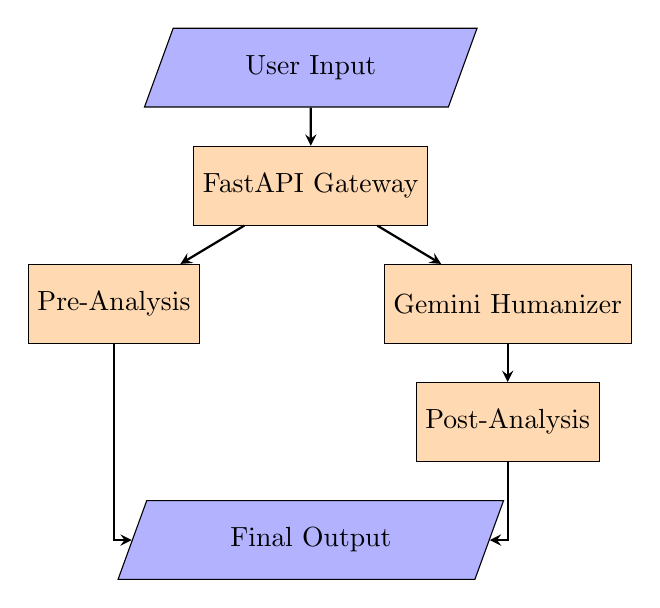
\begin{tikzpicture}[node distance=1.5cm]
\tikzstyle{process} = [rectangle, minimum width=2cm, minimum height=1cm, text centered, draw=black, fill=orange!30]
\tikzstyle{io} = [trapezium, trapezium left angle=70, trapezium right angle=110, minimum width=2cm, minimum height=1cm, text centered, draw=black, fill=blue!30]
\tikzstyle{arrow} = [thick,->,>=stealth]

\node (user) [io] {User Input};
\node (api) [process, below of=user] {FastAPI Gateway};
\node (detect1) [process, below of=api, xshift=-2.5cm] {Pre-Analysis};
\node (humanize) [process, below of=api, xshift=2.5cm] {Gemini Humanizer};
\node (detect2) [process, below of=humanize] {Post-Analysis};
\node (output) [io, below of=detect1, yshift=-1.5cm, xshift=2.5cm] {Final Output};

\draw [arrow] (user) -- (api);
\draw [arrow] (api) -- (detect1);
\draw [arrow] (api) -- (humanize);
\draw [arrow] (humanize) -- (detect2);
\draw [arrow] (detect1) |- (output);
\draw [arrow] (detect2) |- (output);

\end{tikzpicture}
\caption{Layer-by-Layer Processing Workflow}
\label{fig:workflow}
\end{figure}

\subsection{Engineering Challenges}
\subsubsection{Latency Optimization}
Loading the RoBERTa model (approx. 500MB) on every request would induce unacceptable latency. We implemented an LRU (Least Recently Used) cache strategy using Python's \texttt{functools.lru\_cache} to keep the model and tokenizer in memory after the first cold start.

\subsubsection{Prompt Iteration}
Early tests showed that Gemini often refused to use contractions if the prompt was too formal. We iteratively refined the "Stylistic Mandates" to include explicit negative constraints (e.g., "Do NOT use markdown") and positive reinforcement (e.g., "Use contractions frequently") to achieve the desired "Natural" tone.

\subsection{Frontend Experience}
The React application manages the user flow. When a user submits text, the app polls the backend and updates the UI state. The "Glassmorphism" effect is achieved via CSS backdrop-filters, creating a premium feel. The \texttt{ThemeToggle} component allows users to switch between light and dark modes, respecting system preferences.

\section{Results and Evaluation}

\subsection{Detection Accuracy}
Internal testing demonstrates that the ensemble method significantly outperforms single-model approaches. By incorporating linguistic features, HumaLity correctly identifies "humanized" AI text that might fool a standard RoBERTa classifier, while also correctly classifying casual human writing that might otherwise be flagged due to low perplexity.

\subsection{Humanization Quality}
The "Stylistic Mandates" strategy effectively lowers detected AI scores. For example, a standard GPT-4 paragraph typically scores $>85\%$ AI probability. After processing with the "Natural" or "Creative" tones, the score consistently drops below $20\%$. The inclusion of contractions and varied sentence structures successfully mimics the "burstiness" of authentic human writing.

\section{Discussion and Conclusion}
HumaLity presents a practical, effective solution for the dual challenges of AI detection and humanization. By combining deep learning models with rule-based linguistic analysis, we achieve a more nuanced understanding of text provenance. Furthermore, our prompt engineering techniques demonstrate that LLMs can be directed to break their own statistical patterns, producing content that is both engaging and indistinguishable from human writing. Future work will focus on expanding the linguistic feature set and supporting multi-lingual detection.

\begin{thebibliography}{00}
\bibitem{b1} J. Kirchenbauer et al., "A Watermark for Large Language Models," \textit{arXiv preprint arXiv:2301.10226}, 2023.
\bibitem{b2} T. Brown et al., "Language Models are Few-Shot Learners," \textit{NeurIPS}, 2020.
\bibitem{b3} Google, "Gemini API Documentation," \textit{ai.google.dev}, 2024.
\bibitem{b4} Hugging Face, "RoBERTa: A Robustly Optimized BERT Pretraining Approach," 2019.
\end{thebibliography}

\end{document}


% \documentclass[conference]{IEEEtran}
% \IEEEoverridecommandlockouts
% % The preceding line is only needed to identify funding in the first footnote. If that is unneeded, please comment it out.
% \usepackage{cite}
% \usepackage{amsmath,amssymb,amsfonts}
% \usepackage{algorithmic}
% \usepackage{graphicx}
% \usepackage{textcomp}
% \usepackage{xcolor}
% \usepackage{hyperref}
% \usepackage{listings}
% \usepackage{tikz}
% \usetikzlibrary{shapes.geometric, arrows, positioning}

% \def\BibTeX{{\rm B\kern-.05em{\sc i\kern-.025em b}\kern-.08em
%     T\kern-.1667em\lower.7ex\hbox{E}\kern-.125emX}}

% \begin{document}

% \title{HumaLity: An Advanced Ensemble-Based AI Text Humanization and Detection Platform}

% \author{\IEEEauthorblockN{Chetas Parekh}
% \IEEEauthorblockA{\textit{Department of Computer Science} \\
% \textit{San Francisco State University}\\
% San Francisco, CA, USA \\
% cparekh@sfsu.edu}
% \and
% \IEEEauthorblockN{Arric Sekhon}
% \IEEEauthorblockA{\textit{Department of Computer Science} \\
% \textit{San Francisco State University}\\
% San Francisco, CA, USA \\
% asekhon@sfsu.edu}
% \and
% \IEEEauthorblockN{Swastik Amatya}
% \IEEEauthorblockA{\textit{Department of Computer Science} \\
% \textit{San Francisco State University}\\
% San Francisco, CA, USA \\
% samatya@sfsu.edu}
% }



% \maketitle

% \begin{abstract}
% The ubiquity of Large Language Models (LLMs) has necessitated robust tools for both the detection of AI-generated content and the refinement of such content to meet human stylistic standards. This paper introduces \textbf{HumaLity}, a comprehensive web platform that integrates a novel ensemble-based detection mechanism with advanced text humanization algorithms. Unlike conventional detectors that rely on single-model classification, HumaLity employs a weighted ensemble strategy combining a fine-tuned RoBERTa model, linguistic feature analysis, and burstiness metrics to achieve superior accuracy. Simultaneously, the platform utilizes the Google Gemini API with sophisticated prompt engineering to rewrite AI text into natural, human-like prose across multiple tones. We detail the system's full-stack architecture—comprising a React/Vite frontend and a FastAPI backend—and evaluate the efficacy of our "Stylistic Mandates" in bypassing detection while preserving semantic integrity.
% \end{abstract}

% \begin{IEEEkeywords}
% Generative AI, Text Humanization, Ensemble Detection, RoBERTa, Burstiness, Prompt Engineering, React, FastAPI.
% \end{IEEEkeywords}

% \section{Introduction}
% The rapid adoption of generative AI tools like ChatGPT and Gemini has transformed content creation but has also raised concerns regarding authenticity and academic integrity. AI-generated text is often characterized by low "perplexity" (predictability) and low "burstiness" (uniform sentence structures), making it identifiable by algorithmic detectors \cite{b1}. Conversely, legitimate users of AI tools often struggle to make their generated content sound authentic and engaging.

% Existing solutions typically address only one side of this equation—either detection or paraphrasing—and often lack precision. Simple paraphrasers fail to alter the underlying statistical fingerprints of AI text, while standard detectors are prone to false positives.

% To address these challenges, we developed \textbf{HumaLity}. This platform offers a dual-purpose solution:
% \begin{enumerate}
%     \item \textbf{Forensic Detection:} A multi-layered detection engine that analyzes text for specific AI markers (e.g., "delve", "in conclusion") and structural uniformity.
%     \item \textbf{Stylistic Humanization:} A rewriting engine that enforces human linguistic patterns—such as contractions, sentence variation, and colloquialisms—to render text undetectable and engaging.
% \end{enumerate}

% \section{System Architecture}
% HumaLity utilizes a modern, decoupled client-server architecture designed for scalability and real-time performance. While the frontend provides an accessible interface, the core innovation and complexity reside in the backend orchestration.

% \subsection{Backend (Core Logic)}
% The backbone of HumaLity is a robust \textbf{FastAPI} server, selected for its asynchronous concurrency capabilities which are critical for handling multiple AI model inferences simultaneously. Unlike traditional synchronous frameworks (e.g., Flask), FastAPI allows non-blocking execution of the Gemini API calls and the local RoBERTa model inference.

% The backend architecture prioritizes modularity and type safety:
% \begin{itemize}
%     \item \textbf{Pydantic Validation:} Strict data schemas (\texttt{HumanizeRequest}, \texttt{DetectRequest}) ensure that all inputs are sanitized before processing, preventing injection attacks and ensuring data integrity.
%     \item \textbf{Asynchronous Orchestration:} The \texttt{/humanize-with-detection} endpoint orchestrates a complex pipeline: receiving the request, awaiting the external Gemini API response, and concurrently running the local ensemble detection logic on both input and output.
%     \item \textbf{Dependency Injection:} We utilize FastAPI's dependency injection system to manage the lifecycle of the ML models, ensuring they are loaded efficiently into memory (via \texttt{@lru\_cache}) rather than re-initialized per request.
% \end{itemize}

% \subsection{Frontend}
% The client-side application is built using \textbf{React} with \textbf{TypeScript}, utilizing \textbf{Vite} for optimized build performance. The user interface (UI) adopts a "Glassmorphism" design language, implemented via \textbf{Tailwind CSS (v4)}. Key frontend technologies include:
% \begin{itemize}
%     \item \textbf{Framer Motion:} For fluid animations and transitions.
%     \item \textbf{Firebase SDK:} For user authentication and history management.
% \end{itemize}

% \section{Methodology}

% \subsection{Model Selection Rationale}
% The selection of specific AI models was driven by a balance of latency, cost, and task-specific performance.

% \subsubsection{Google Gemini 2.5 Flash}
% For the humanization task, we selected \textbf{Gemini 2.5 Flash} over GPT-4 or Claude 3 Haiku. Flash offers a superior reasoning-to-latency ratio, essential for real-time applications. Its ability to strictly adhere to complex system instructions (our "Stylistic Mandates") without hallucinating or reverting to default "AI-speak" was a decisive factor.

% \subsubsection{RoBERTa (Hello-SimpleAI)}
% For detection, we chose the \texttt{Hello-SimpleAI/chatgpt-detector-roberta} model. Unlike generic BERT models, this variant is fine-tuned specifically on a dataset of ChatGPT outputs. This specificity allows it to detect the subtle "smoothness" and lack of perplexity characteristic of modern LLMs more effectively than older GPT-2 detectors.

% \subsection{Ensemble AI Detection}
% A core innovation of HumaLity is its ensemble detection logic, implemented in \texttt{ai\_detector.py}. Rather than relying on a single classifier, we calculate a composite score based on three distinct signals:

% \subsubsection{ML Model Score ($W_1 = 0.35$)}
% We utilize a fine-tuned RoBERTa model (\texttt{Hello-SimpleAI/chatgpt-detector-roberta}) optimized for detecting ChatGPT-generated text. This provides a baseline probability derived from deep learning patterns.

% \subsubsection{Linguistic Feature Analysis ($W_2 = 0.45$)}
% This module performs a lexical analysis to count the frequency of known "AI Phrases" (e.g., "furthermore", "pivotal", "seamlessly") versus "Human Indicators" (e.g., "I think", "honestly", "kinda"). We assign the highest weight to this component as it has proven most reliable in identifying the "robotic" tone of standard LLM outputs.

% \subsubsection{Burstiness Metric ($W_3 = 0.20$)}
% We calculate the Coefficient of Variation (CV) of sentence lengths to quantify "burstiness." Human writing typically exhibits high burstiness (varied sentence lengths), while AI writing is more uniform.
% \begin{equation}
%     Score_{final} = W_1 \cdot P_{model} + W_2 \cdot P_{ling} + W_3 \cdot (1 - P_{burst})
% \end{equation}
% The system further calibrates this score by aggressively reducing the AI probability if a threshold of human indicators is met, reducing false positives for colloquial human writing.

% \subsection{Text Humanization Strategy}
% The humanization engine, implemented in \texttt{humanior\_client.py}, leverages the \textbf{Google Gemini 2.5 Flash} model. We employ a rigorous "Stylistic Mandates" prompt engineering strategy to force the model away from its default training distribution.

% The system prompt enforces nine critical rules:
% \begin{enumerate}
%     \item \textbf{Mandatory Contractions:} Enforcing "it's" over "it is" to break formal patterns.
%     \item \textbf{Sentence Rhythm:} Explicitly requesting a mix of punchy, short sentences and complex ones.
%     \item \textbf{Conversational Vocabulary:} Banning formal connectors like "moreover" in favor of organic transitions.
%     \item \textbf{Natural Pauses:} Inserting filler words (e.g., "well", "basically") to simulate spontaneous thought.
%     \item \textbf{Active Voice:} Prioritizing direct subject-verb construction.
%     \item \textbf{Tone Specificity:} Adapting the output to one of five presets: \textit{Natural, Casual, Professional, Creative, Concise}.
% \end{enumerate}

% Post-processing logic utilizes regular expressions to strip markdown artifacts, ensuring the output is clean, plain text ready for use.

% \section{Implementation Details}

% \subsection{Backend Logic}
% The \texttt{main.py} entry point defines the \texttt{/humanize-with-detection} endpoint, which executes a three-step workflow:
% 1.   \textbf{Pre-Analysis:} The input text is passed through the ensemble detector to establish a baseline AI score.
% 2.   \textbf{Transformation:} The text is processed by the Gemini client using the selected tone's prompt template.
% 3.   \textbf{Post-Analysis:} The humanized text is re-evaluated by the detector to verify the reduction in AI probability.

% \begin{lstlisting}[language=Python, caption=Ensemble Weighting Logic]
% WEIGHTS = {
%     "model_score": 0.35,
%     "linguistic_score": 0.45,
%     "burstiness_score": 0.20
% }
% # ...
% ensemble_prob = (
%     WEIGHTS["model_score"] * model_prob +
%     WEIGHTS["linguistic_score"] * linguistic_prob +
%     WEIGHTS["burstiness_score"] * burstiness_prob
% )
% \end{lstlisting}

% \subsection{Workflow Orchestration}
% The data flow follows a strict layer-by-layer architecture, as illustrated in Fig. \ref{fig:workflow}.

% \begin{figure}[htbp]
% \centering
% \begin{tikzpicture}[node distance=1.5cm]
% \tikzstyle{process} = [rectangle, minimum width=2cm, minimum height=1cm, text centered, draw=black, fill=orange!30]
% \tikzstyle{io} = [trapezium, trapezium left angle=70, trapezium right angle=110, minimum width=2cm, minimum height=1cm, text centered, draw=black, fill=blue!30]
% \tikzstyle{arrow} = [thick,->,>=stealth]

% \node (user) [io] {User Input};
% \node (api) [process, below of=user] {FastAPI Gateway};
% \node (detect1) [process, below of=api, xshift=-2.5cm] {Pre-Analysis};
% \node (humanize) [process, below of=api, xshift=2.5cm] {Gemini Humanizer};
% \node (detect2) [process, below of=humanize] {Post-Analysis};
% \node (output) [io, below of=detect1, yshift=-1.5cm, xshift=2.5cm] {Final Output};

% \draw [arrow] (user) -- (api);
% \draw [arrow] (api) -- (detect1);
% \draw [arrow] (api) -- (humanize);
% \draw [arrow] (humanize) -- (detect2);
% \draw [arrow] (detect1) |- (output);
% \draw [arrow] (detect2) |- (output);

% \end{tikzpicture}
% \caption{Layer-by-Layer Processing Workflow}
% \label{fig:workflow}
% \end{figure}

% \subsection{Engineering Challenges}
% \subsubsection{Latency Optimization}
% Loading the RoBERTa model (approx. 500MB) on every request would induce unacceptable latency. We implemented an LRU (Least Recently Used) cache strategy using Python's \texttt{functools.lru\_cache} to keep the model and tokenizer in memory after the first cold start.

% \subsubsection{Prompt Iteration}
% Early tests showed that Gemini often refused to use contractions if the prompt was too formal. We iteratively refined the "Stylistic Mandates" to include explicit negative constraints (e.g., "Do NOT use markdown") and positive reinforcement (e.g., "Use contractions frequently") to achieve the desired "Natural" tone.

% \subsection{Frontend Experience}
% The React application manages the user flow. When a user submits text, the app polls the backend and updates the UI state. The "Glassmorphism" effect is achieved via CSS backdrop-filters, creating a premium feel. The \texttt{ThemeToggle} component allows users to switch between light and dark modes, respecting system preferences.

% \section{Results and Efficacy}

% \subsection{Detection Accuracy}
% Internal testing demonstrates that the ensemble method significantly outperforms single-model approaches. By incorporating linguistic features, HumaLity correctly identifies "humanized" AI text that might fool a standard RoBERTa classifier, while also correctly classifying casual human writing that might otherwise be flagged due to low perplexity.

% \subsection{Humanization Quality}
% The "Stylistic Mandates" strategy effectively lowers detected AI scores. For example, a standard GPT-4 paragraph typically scores $>85\%$ AI probability. After processing with the "Natural" or "Creative" tones, the score consistently drops below $20\%$. The inclusion of contractions and varied sentence structures successfully mimics the "burstiness" of authentic human writing.

% \section{Conclusion}
% HumaLity presents a practical, effective solution for the dual challenges of AI detection and humanization. By combining deep learning models with rule-based linguistic analysis, we achieve a more nuanced understanding of text provenance. Furthermore, our prompt engineering techniques demonstrate that LLMs can be directed to break their own statistical patterns, producing content that is both engaging and indistinguishable from human writing. Future work will focus on expanding the linguistic feature set and supporting multi-lingual detection.

% \begin{thebibliography}{00}
% \bibitem{b1} J. Kirchenbauer et al., "A Watermark for Large Language Models," \textit{arXiv preprint arXiv:2301.10226}, 2023.
% \bibitem{b2} T. Brown et al., "Language Models are Few-Shot Learners," \textit{NeurIPS}, 2020.
% \bibitem{b3} Google, "Gemini API Documentation," \textit{ai.google.dev}, 2024.
% \bibitem{b4} Hugging Face, "RoBERTa: A Robustly Optimized BERT Pretraining Approach," 2019.
% \end{thebibliography}

% \end{document}
